
%%% Local Variables: 
%%% mode: latex
%%% TeX-master: "main"
%%% End: 

% This section describes the prevalence of the background signal
% Showing specific examples of the background signal and promoter prevalence

\subsubsection{Background Signal}
\begin{wrapfigure}{l}{0.4\textwidth}
\small
\vspace{-20pt}
\begin{center}
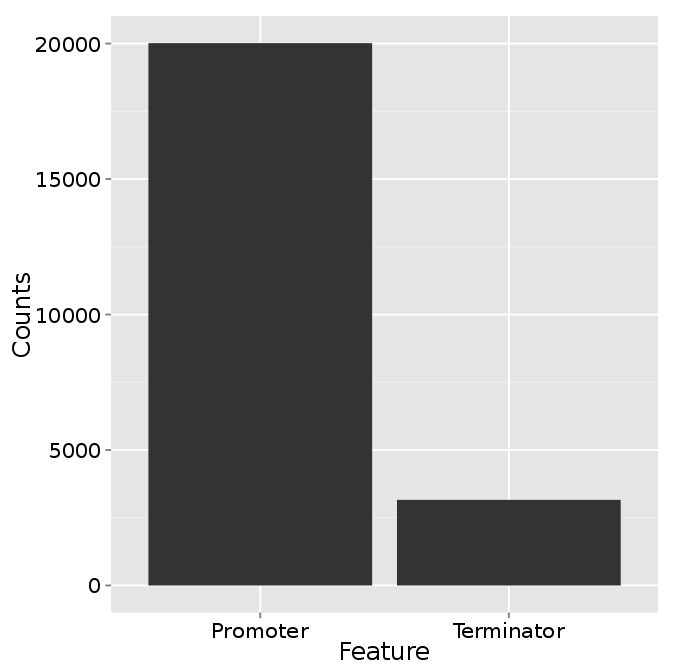
\includegraphics[width=0.38\textwidth]{images/Assembly/Background_signal/prediction_frequency.png}
\end{center}
\vspace{-20pt}
\caption{Feature Frequency}\label{fig:5.6}
\end{wrapfigure}

A large number of Sigma A promoters were predicted (\ref{fig:5.6}), close to 3x the number of predicted terminators, throughout the \textit{C. acetobutylicum} genome. These promoters are uniformly distributed throughout the genome and are not necessarily concentrated at the beginning of transcripts (\ref{fig:5.7}). Many of these predictions were weak matches to the consensus motifs and would have only weak affinity for $\sigma$-factors, producing only residual transcriptional activity. The AT-rich genome of \textit{C. acetobutylicum} leads to an abundance of putative promoter sequences, contributing to the background signal observed both statistically and through specific examples (\ref{fig:5.8}). A side benefit of promoter prediction was the quantification of their prevalence, which may contribute to the observed background signal. As we will see shortly, integrating these promoter motifs with the assembly dataset also helped resolve misassemblies and ambiguous boundaries. 


\begin{figure}
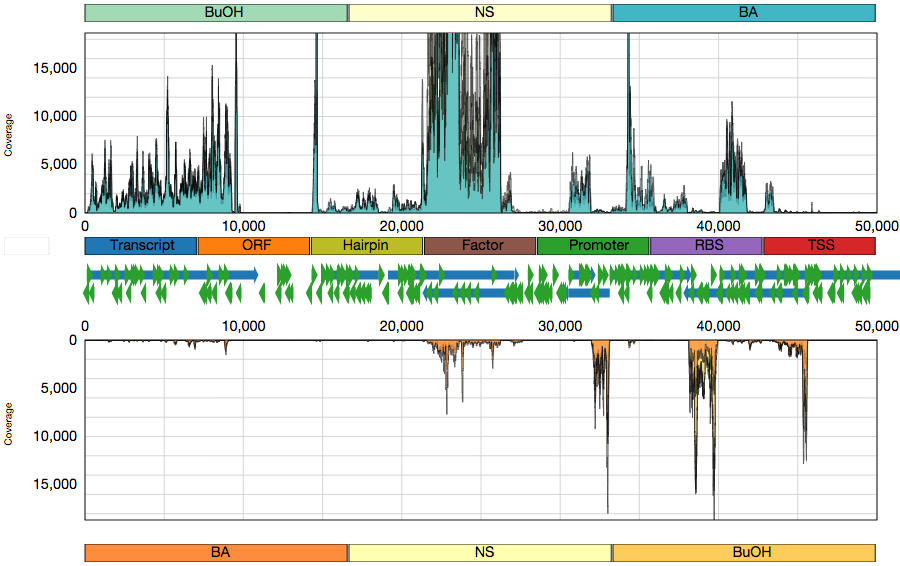
\includegraphics[width=\textwidth]{images/Assembly/Background_signal/promoter_prevalence.png}
\caption{Promoter Prevalence}\label{fig:5.7}
\end{figure}



\begin{figure}
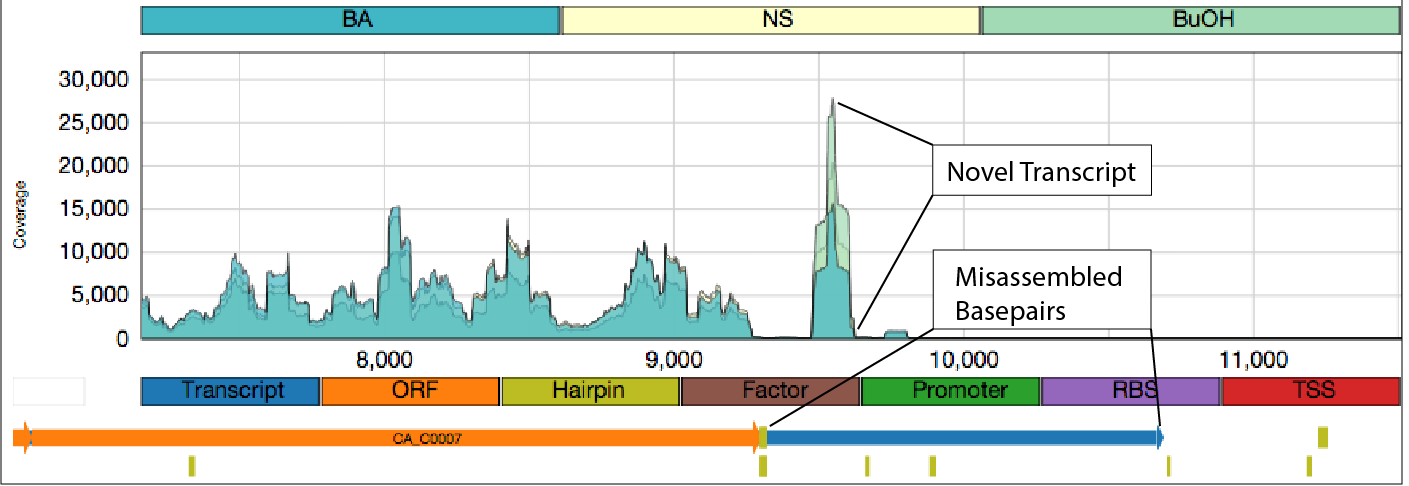
\includegraphics[width=\textwidth]{images/Assembly/Background_signal/Background_signal.png}
\caption{Background Signal}\label{fig:5.8}
\end{figure}


The transcriptome assembly was inspected with the customized genome browser to understand this background signal and determine if the transcript boundary estimates could be improved by curation. The assembled transcripts matched the sequencing depth well, despite the misassemblies that were apparent upon examination (\ref{fig:5.8}). Assembly extended through some troughs in depth (transcript fusion) and beyond expression termini (transcript extension). The extent of background signal - residual depth in seemingly inactive regions of the genome - is impossible to quantify without first distinguishing true signal from the noise through assembly curation. With existing technologies, some background signal is expected (ENCODE reference) and this complicated the process of assembly and curation.

Potential sources for this noise include residual antisense signal (1-5\%), contaminating DNA, and spurious transcription, minor signals that can be minimized in some ways but are difficult to eliminate in RNA sequencing experiments. Residual antisense signal is a factor of the library preparation method. This particular signal was not overly abundant (1-5\%, refernce strand specific review) and was carefully considered during curation in each case of antisense transcription. Contaminating DNA was minimized through filtration and enzymatic removal steps in this work; also, contaminating DNA was not observed during quality control checkpoints. While residual contaminants might have contributed towards the background signal, we would expect that their effect was minimal and their contribution would have been uniform throughout the genome. It is reasonable to suspect that these signals produced a small, predictably uniform background signal in the genome.

The last source, spurious transcription, can be minimized through certain extraction and size selection techniques during library preparation. However, this experiment was designed to identify all coding and noncoding primary transcripts. The RNA extraction technique used (methods rna extraction) does not exclude short transcripts, such as those from non-specific transcription. The previously described sequencing depth suggested that some of this signal was expected (ENCODE reference). Spurious transcription is also supported by the promoter prediction frequency observed throughout the genome (\ref{fig:5.6}) and the uniform distribution of these motifs in both transcribed and untranscribed regions of the genome (\ref{fig:5.7}). Similarly to the other contributors, a small and uniform noise is expected given the extreme sequencing depth, and this noise is the most likely cause of misassembly.


 Fortunately, there were distinct depth patterns (\ref{fig:5.8}) that agree with promoter and terminator annotations. The separation of true signal from noise was possible by integrating these multiple datasets through the genome browser. Next, the curation process is detailed for specific examples, where previous gene-specific experiments have produced transcript boundaries. The integrated analysis corrected for these background signals, revealing precise and accurate estimates of transcript boundaries. 



